\documentclass[11pt, twoside]{article}   	% use "amsart" instead of "article" for AMSLaTeX format
\usepackage{geometry}                		% See geometry.pdf to learn the layout options. There are lots.
\geometry{a4paper}                   		% ... or a4paper or a5paper or ... 
\linespread{1.0}
%\geometry{landscape}                		% Activate for rotated page geometry
%\usepackage[parfill]{parskip}    		% Activate to begin paragraphs with an empty line rather than an indent
\usepackage{graphicx}				% Use pdf, png, jpg, or eps§ with pdflatex; use eps in DVI mode
								% TeX will automatically convert eps --> pdf in pdflatex		

\pagestyle{headings}

%SetFonts

\usepackage{mathrsfs}
\usepackage{amsthm, amsmath, amssymb}

\usepackage{unicode-math}
%\usepackage{fourier}
%\usepackage{fontspec}
%\setmathfont{STIX Two Math}
%\setmathfont{STIX Two Math}[StylisticSet = 1, range = scr]
%\setmathrm{STIX Two Math}
%\usepackage{newpxmath}
%\setmainfont{Scala}
%\setmonofont{SF Mono}
\usepackage{xeCJK}
\usepackage{bbold}

\usepackage{graphicx}

\def\rcurs{{\mbox{$\resizebox{.16in}{.08in}{\includegraphics{ScriptR}}$}}}
\def\brcurs{{\mbox{$\resizebox{.16in}{.08in}{\includegraphics{BoldR}}$}}}
\def\hrcurs{{\mbox{$\hat \brcurs$}}}

\usepackage{color, xcolor}
\usepackage{ebezier}
\usepackage{tikz}
\usepackage{circuitikz}
\usepackage{physics2}
\usephysicsmodule{ab, braket, bm-um.legacy, diagmat}

\usepackage[colorlinks,
linkcolor = blue,
anchorcolor = blue,
citecolor = blue,
urlcolor = blue]{hyperref}

\usepackage{multirow}
\usepackage{makecell}
\usepackage{booktabs}
\usepackage{wrapfig}
\usepackage{caption}
\usepackage{lastpage}

\usepackage{appendix}
\theoremstyle{plain}
\newtheorem{lemma}{Lemma}[section]
\newtheorem{theorem}[lemma]{Theorem}
\newtheorem{axiom}[lemma]{Axiom}
\newtheorem{corollary}[lemma]{Corollary}
\newtheorem{proposition}[lemma]{Proposition}
\theoremstyle{definition}
\newtheorem{definition}[lemma]{Definition}
\newtheorem{remark}{Remark}[section]
\newtheorem{example}[lemma]{Example}

\usepackage{syntonly}
%\syntaxonly

\usepackage{fancyhdr}
\pagestyle{fancy}
\fancyhf{}
\fancyhead[R]{黄远墨 \textsf{2023141220092}}
\fancyhead[L]{第六章习题}
\fancyfoot[C]{\thepage/\pageref{LastPage}}
\renewcommand{\headrulewidth}{0.5pt}

%\renewcommand{\footrulewidth}{0.5pt}

\title{Homework}
\author{黄远墨 2023141220092}
\date{}							% Activate to display a given date or no date

\begin{document}
	% generates the title
	%\maketitle
	\thispagestyle{fancy}
	\section{Problem 6}
	
	\begin{description}
		\item[6.1] $R / \lambda \ll L / R \quad \Rightarrow \quad L \approx 10 R^2 / \lambda = 24.69
			\mathrm{m}$.
		\item[6.2] $E(\theta) = \frac{E_0}{\int_{-a/2}^{a/2} \cos(\pi x / a) \mathrm{d}x} \mathcal F \left\{ t(x) \right\} = \frac{\pi E_0}{2 a} \int_{-a/2}^{a/2} \cos(\pi x / a) \mathrm e^{\mathrm{i} k x \sin\theta} \mathrm{d}x \quad \Rightarrow$
			\begin{equation}
				E(u) = E_0 \frac{\cos u}{1 - \frac{4}{\pi^2} u^2} = \frac{\pi E_0}{4} \left( \frac{\sin(u - \pi/2)}{u - \pi / 2} + \frac{\sin(u + \pi / 2)}{u + \pi / 2} \right),
			\end{equation}
			$u = \frac{\pi a}{\lambda} \sin\theta$. 无膜片:
			\begin{equation}
				E_s(u) = \frac{E_0}{a} \int_{-a/2}^{a/2} \mathrm e^{\mathrm{i} k \sin\theta} \mathrm{d}x = E_0 \frac{\sin u}{u}.
			\end{equation}
			则
			\begin{equation}
				E(u) = \frac{\pi}{4} \left[ E_s(u - \pi / 2) + E_s(u + \pi / 2) \right].
			\end{equation}
		\item[6.4] 令
			\begin{equation}
				s(x) = \sum_{n = 0}^{N-1} \delta(x - (n - \tfrac{N - 1}{2}) d), \quad
				t(x) =
				\begin{cases}
					1, & x \leq a / 2,\\
					0, & x > a / 2.
				\end{cases}
			\end{equation}
			则
			\begin{align}
				\mathcal F\{s\} &= \int_{-\infty}^{\infty} s(x) \mathrm e^{\mathrm{i}kx\sin\theta} \mathrm{d}x = \frac{\sin\left(N \frac{\pi d}{\lambda} \sin\theta \right)}{\sin\left( \frac{\pi d}{\lambda} \sin\theta \right)},\\
				\mathcal F\{t\} &= \int_{-\infty}^{\infty} t(x) \mathrm e^{\mathrm{i}kx\sin\theta} \mathrm{d}x = a \frac{\sin\left( \frac{\pi a}{\lambda} \sin\theta \right)}{\frac{\pi a}{\lambda} \sin\theta}.
			\end{align}
			光栅函数为 $(s * t)(x) := \int_{-\infty}^{\infty} s(t) t(x - t) \mathrm{d}t$, 故光场
			\begin{equation}
				E(\theta) = \mathcal F\{s * t\} = \mathcal F\{s\} \cdot \mathcal F\{t\},
			\end{equation}
			光强
			\begin{equation}
				I(\theta) = E^2(\theta) = a^2 \frac{\sin^2 \left( \frac{\pi a}{\lambda} \sin\theta \right)}{\left( \frac{\pi a}{\lambda} \sin\theta \right)^2} \frac{\sin^2 \left( N \frac{\pi d}{\lambda} \sin\theta \right)}{\sin^2 \left( \frac{\pi d}{\lambda} \sin\theta \right)}.
			\end{equation}
		\item[6.6] $\theta \leq r / d \quad \Rightarrow \quad f = \theta / \lambda \leq \frac{r}{\lambda d}$.
		\item[6.8] 设焦距为 $f$, 口径为 $D$. 光栅常数 $d = 10^{-5} \mathrm{m}$, $2 \mathrm{mm} / f = \lambda / d \Rightarrow f = 2 \mathrm{mm} \cdot d / \lambda = 31.6 \mathrm{mm}$. $\frac{D/2}{f} \geq 5\lambda / d \Rightarrow D \geq 10 \lambda f / d = 20 \mathrm{mm}$.

			\section{Simulation}
			设物屏坐标为 $x, y$, 像屏坐标为 $X, Y$, 像屏与物屏相距 $D$,
			\begin{equation}
				E(X, Y) = \frac{E_0}{a^2} \int_{-\infty}^{\infty} \mathrm{d}x \int_{-\infty}^{\infty} \mathrm{d}y f(x, y) \mathrm e^{\mathrm{i}\frac{k}{D} (xX + yY)},
			\end{equation}
			其中
			\begin{equation}
				f(x, y) = (s_{d_x} * t)(x) \cdot (s_{d_y} * t)(y).
			\end{equation}
			计算得
			\begin{equation}
				E(X, Y) = E_0 \frac{\sin \left( \frac{\pi a}{\lambda D} X \right)}{\frac{\pi a}{\lambda D} X} \frac{\sin \left( \frac{\pi a}{\lambda D} Y \right)}{\frac{\pi a}{\lambda D} Y} \frac{\sin \left( N \frac{\pi d_x}{\lambda D} X \right)}{\sin \left( \frac{\pi d_x}{\lambda D} X \right)} \frac{\sin \left( N \frac{\pi d_y}{\lambda D} Y \right)}{\sin \left( \frac{\pi d_y}{\lambda D} Y \right)}.
			\end{equation}
			下面画出 $E^2(X, Y)$ 的分布.

			\begin{figure}[htbp]
				\begin{minipage}[t]{0.32\linewidth}
				\centering
				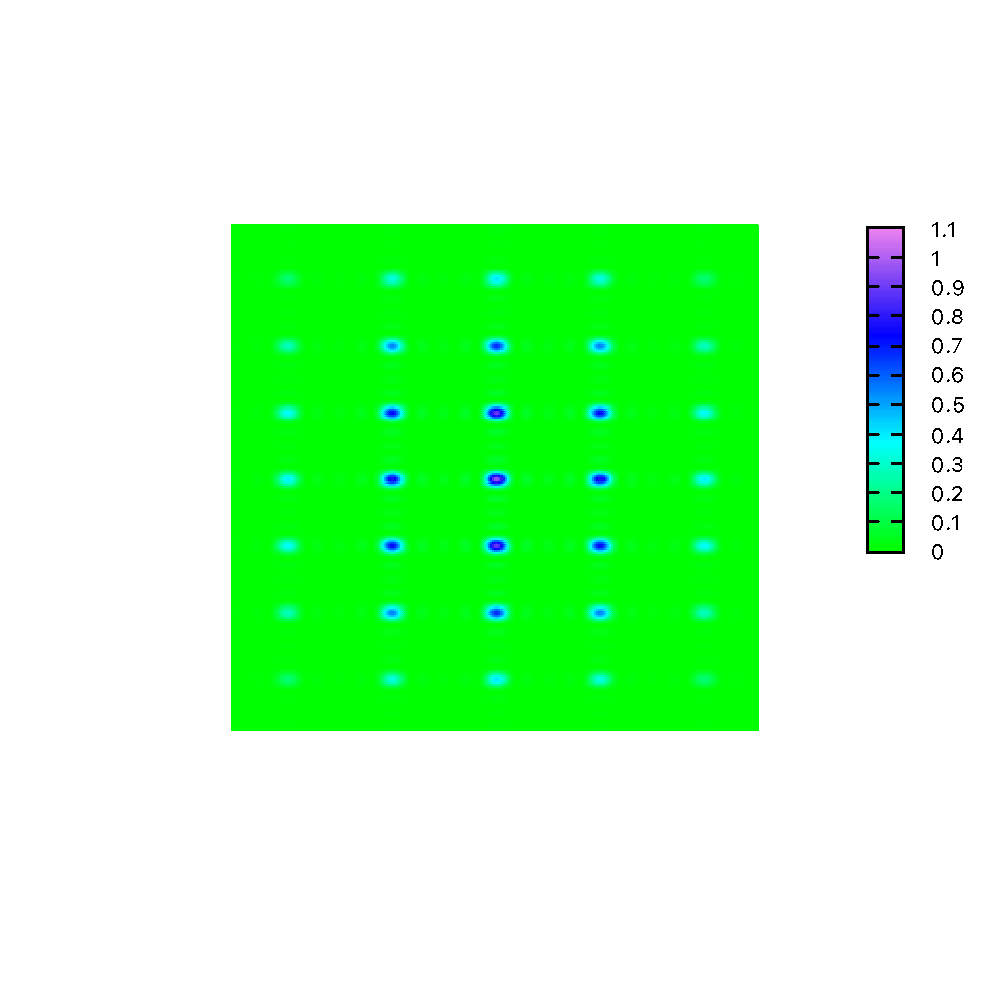
\includegraphics[width=0.9\linewidth]{20-30}
				\captionsetup{font={footnotesize}}
				\caption{$d_x = 20 \mathrm{\mu m}$,\\$d_y = 30 \mathrm{\mu m}$.}
				\end{minipage}
				\begin{minipage}[t]{0.32\linewidth}
				\centering
				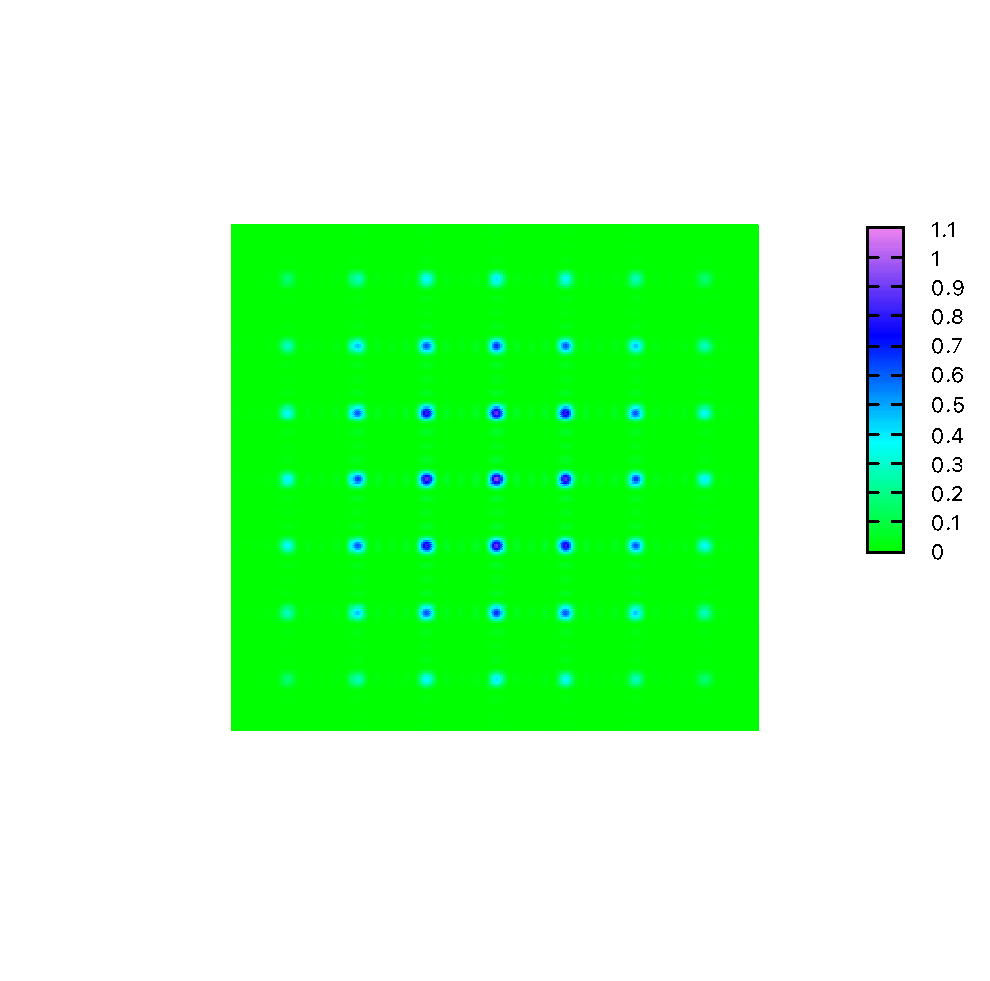
\includegraphics[width=0.9\linewidth]{30-30}
				\captionsetup{font={footnotesize}}
				\caption{$d_x = 30 \mathrm{\mu m}$,\\$d_y = 30 \mathrm{\mu m}$.}
				\end{minipage}
				\begin{minipage}[t]{0.32\linewidth}
				\centering
				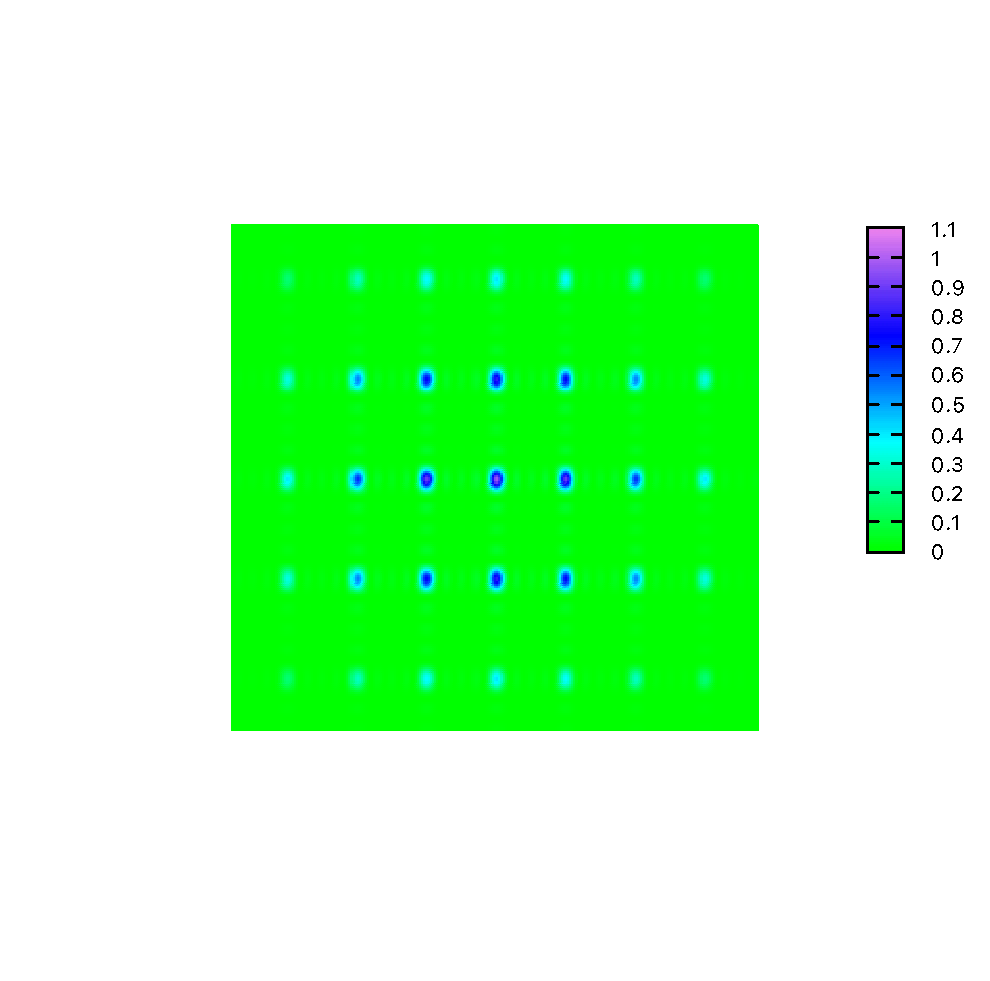
\includegraphics[width=0.9\linewidth]{30-20}
				\captionsetup{font={footnotesize}}
				\caption{$d_x = 30 \mathrm{\mu m}$,\\$d_y = 20 \mathrm{\mu m}$.}
				\end{minipage}
			\end{figure}
		\end{description}
	
\end{document}


